\documentclass[12pt]{article}                         
\pagestyle{plain} %-- Document Set Up Command

%-- Document Setup & Layout
\usepackage{fancyhdr}
\usepackage{comment}
\usepackage{multicol}
\usepackage[
  letterpaper,
  left=0.8in,
  right=0.8in,
  textheight=9.5in,
  bmargin=0.75in  % Adjust this value to push the footer down
]{geometry}

%-- Color & Text Formatting
\usepackage[svgnames]{xcolor} 
\usepackage{textcomp}
\usepackage{ulem}
\usepackage{graphicx}

%-- Math Packages
\usepackage{amsmath}     
\usepackage{amsfonts}
\usepackage{amstext}
\usepackage{amssymb}
\usepackage{latexsym}
\usepackage{bm}

%-- Graphics and Figures
\usepackage{graphicx}    
\usepackage{tikz}
\usepackage{pgfplots}
\usepackage{circledtext}
\usepackage{float}
\usepackage{caption}
\usepackage{subcaption}
\usetikzlibrary{decorations.markings, arrows.meta}
%-- Tables
\usepackage{array}      
\usepackage{tabularx}

%-- Lists
\usepackage{enumitem}    
%\usepackage{enumerate}
\usepackage{tasks}

%-- TikZ Libraries
\usetikzlibrary{shapes.geometric} 
\pgfplotsset{compat=1.18}

\tikzset{
    phase arrow right/.style={
        postaction={decorate,
            decoration={
                markings,
                mark=at position 0.4 with {\arrow{Stealth}},
                mark=at position 0.9 with {\arrow{Stealth}}
            }
        }
    },
    phase arrow left/.style={
        postaction={decorate,
            decoration={
                markings,
                mark=at position 0.4 with {\arrow{Stealth[reversed]}},
                mark=at position 0.9 with {\arrow{Stealth[reversed]}}
            }
        }
    }
}
%-- Header/Footer
\pagestyle{fancy}
\fancyhf{} % Clear all header and footer fields
\fancyhead[L]{Jack Lingbeck} % Left header with name
\fancyhead[R]{February 10th, 2026} % Right header with date
\renewcommand{\headrulewidth}{0.4pt} % Horizontal line below the header
\rfoot{Page \thepage}
\lfoot{Homework 2}

\begin{document}
\large
\begin{center}
\fbox{\begin{tabular}{c}
\bf Math 675 Spring 2026: \\
\bf Homework 3 (LATE) \\
\bf Due Tuesday, February 10th, 2026\\
\end{tabular}}
\end{center}

\section*{Question 1:}
\renewcommand{\arraystretch}{1.3}
\begin{enumerate}
\item[a)] $\mathbf{x'} = \begin{pmatrix} \frac{5}{4} & \frac{3}{4} \\ \frac{3}{4} & \frac{5}{4} \end{pmatrix} \mathbf{x}$ \\
    $\left| \begin{array}{cc} \frac{5}{4} - \lambda & \frac{3}{4}\\ \frac{3}{4} & \frac{5}{4} - \lambda\end{array}\right| 
    = \left(\frac{5}{4} - \lambda\right)^2 - \left(\frac{3}{4}\right)^2 = 0 \\\\
    \hspace*{95pt} = \left(\frac{5}{4} - \lambda + \frac{3}{4}\right)\left(\frac{5}{4} - \lambda - \frac{3}{4}\right) = 0 \\\\
    \hspace*{95pt} = \left(2 - \lambda\right)\left(\frac{1}{2} - \lambda\right) = 0 \\\\
    \hspace*{95pt} \Rightarrow \lambda_1 = 2, \lambda_2 = \frac{1}{2}$

    \subsubsection*{Eigenvalue \#1}
    $\mathbf{\lambda_1 = \phantom{-}2}: 
    \left[\begin{array}{cc} \frac{5}{4} - \lambda_1 & \frac{3}{4}\\ \frac{3}{4} & \frac{5}{4} - \lambda_1\end{array}\right]
    \rightarrow \left[\begin{array}{rr} -\frac{3}{4}& \frac{3}{4}\\ \frac{3}{4} & -\frac{3}{4} \end{array}\right] \left[\begin{array}{cc} v_1 \\ v_2 \end{array}\right] = \left[\begin{array}{cc} 0 \\ 0 \end{array}\right]$

    $\hspace*{2cm}\begin{array}{rr} -1v_1 + 1v_2 &=0 \\ 1v_1 - 1v_2 &=0 \end{array} 
     \longrightarrow \quad v_1=v_2 \quad \longrightarrow \mathbf{v}_1 =\left[\begin{array}{cc} 1 \\ 1 \end{array}\right]$

    \subsubsection*{Eigenvalue \#2}
    $\mathbf{\lambda_2 = \phantom{-}\dfrac{1}{2}}: 
    \left[\begin{array}{cc} \frac{5}{4} - \lambda_2 & \frac{3}{4}\\ \frac{3}{4} & \frac{5}{4} - \lambda_2\end{array}\right]
    \rightarrow \left[\begin{array}{rr} \frac{3}{4}& \frac{3}{4}\\ \frac{3}{4} & \frac{3}{4} \end{array}\right] \left[\begin{array}{cc} v_1 \\ v_2 \end{array}\right] = \left[\begin{array}{cc} 0 \\ 0 \end{array}\right]$

    $\hspace*{2cm}\begin{array}{rr} 1v_1 + 1v_2 &=0 \\ 1v_1 + 1v_2 &=0 \end{array} 
    \longrightarrow \quad v_1=-v_2 \quad \longrightarrow \mathbf{v}_2 =\left[\begin{array}{cc} -1 \\ 1 \end{array}\right]$

    \vspace{2cm}

    So our general solution is $\mathbf{x} = c_1\begin{pmatrix} 1 \\ 1 \end{pmatrix}e^{2t} + c_2\begin{pmatrix} -1 \\ 1 \end{pmatrix}e^{\frac{1}{2}t}$
    \\\\
    If we take the limit as $t$ approaches infinity, we can notice both terms head to infinity, but notice that the dominant term is the one with $\lambda_1 = 2$, \\ so all trajectories will be parellel to the line $y = x$ \\
    \begin{figure}[H]
        \centering
        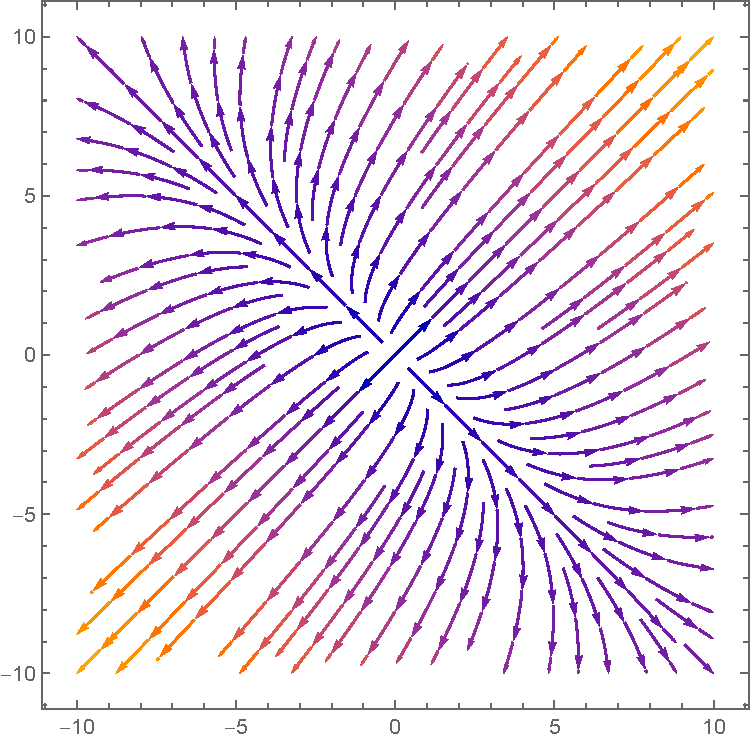
\includegraphics[width=0.4\textwidth]{Homework_3_Images/HW_3_Q1a.pdf}
    \end{figure}
    \vspace{12cm}


\item[b)] $\mathbf{x'} = \begin{pmatrix} 4 & -3\\ 8 & -6 \end{pmatrix} \mathbf{x}$\\
    $\left| \begin{array}{cc} 4 - \lambda & -3\\ 8 & -6 - \lambda\end{array}\right| 
    = (4 - \lambda)(-6 - \lambda) - (-3)(8) = 0 \\\\
    \hspace*{108pt} = -24 - 4\lambda + 6\lambda + \lambda^2 + 24 = 0 \\\\
    \hspace*{108pt} = \lambda^2 + 2\lambda = 0 \\\\
    \hspace*{108pt} \Rightarrow \lambda_1 = 0, \lambda_2 = -2$

    \subsubsection*{Eigenvalue \#1}
    $\mathbf{\lambda_1 = \phantom{-}0}: 
    \left[\begin{array}{cc} 4 - \lambda_1 & -3\\ 8 & -6 - \lambda_1\end{array}\right]
    \rightarrow \left[\begin{array}{rr} 4 & -3\\ 8 & -6 \end{array}\right] \left[\begin{array}{cc} v_1 \\ v_2 \end{array}\right] = \left[\begin{array}{cc} 0 \\ 0 \end{array}\right]$

    $\hspace*{2.2cm}\begin{array}{rr} 4v_1 - 3v_2 &=0 \\ 8v_1 - 6v_2 &=0 \end{array} 
     \longrightarrow \quad 4v_1=3v_2 \quad \longrightarrow \mathbf{v}_1 =\left[\begin{array}{cc} 3 \\ 4 \end{array}\right]$

    \subsubsection*{Eigenvalue \#2}
    $\mathbf{\lambda_2 = -2}: 
    \left[\begin{array}{cc} 4 - \lambda_2 & -3\\ 8 & -6 - \lambda_2\end{array}\right]
    \rightarrow \left[\begin{array}{rr} 6 & -3\\ 8 & -4 \end{array}\right] \left[\begin{array}{cc} v_1 \\ v_2 \end{array}\right] = \left[\begin{array}{cc} 0 \\ 0 \end{array}\right]$

    $\hspace*{2.2cm}\begin{array}{rr} 6v_1 - 3v_2 &=0 \\ 8v_1 - 4v_2 &=0 \end{array} 
    \longrightarrow \quad 2v_1=v_2 \quad \longrightarrow \mathbf{v}_2 =\left[\begin{array}{cc} 1 \\ 2 \end{array}\right]$

    \vspace{6cm}

    So our general solution is $\mathbf{x} = c_1\begin{pmatrix} 1 \\ 1 \end{pmatrix}e^{2t} + c_2\begin{pmatrix} -1 \\ 1 \end{pmatrix}e^{\frac{1}{2}t}$
    \\\\
    If we take the limit as $t$ approaches infinity, we can notice both terms head to infinity, but notice that the dominant term is the one with $\lambda_1 = 2$, \\ so all trajectories will be parellel to the line $y = x$ \\
    \begin{figure}[H]
        \centering
        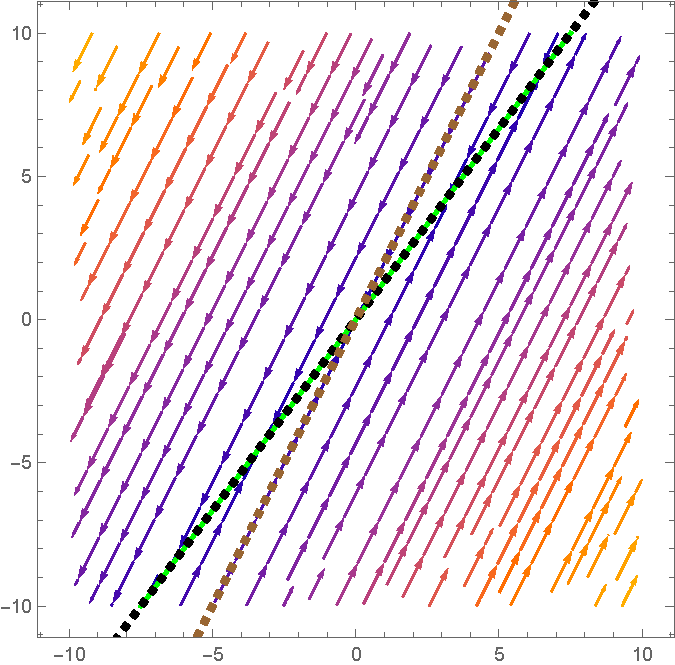
\includegraphics[width=0.4\textwidth]{Homework_3_Images/HW_3_Q1b.pdf}
    \end{figure}
    \vspace{12cm}


\item[c)] $\mathbf{x'} = \begin{pmatrix} 3 & -2 \\ 4 & -1 \end{pmatrix} \mathbf{x}$\\
    $\left| \begin{array}{cc} 3 - \lambda & -2\\ 4 & -1 - \lambda\end{array}\right| 
    = (3 - \lambda)(-1 - \lambda) - (-2)(4) = 0 \\\\
    \hspace*{95pt} = -3 - 3\lambda + \lambda + \lambda^2 + 8 = 0 \\\\
    \hspace*{95pt} = \lambda^2 - 2\lambda + 5 = 0 \\\\
    \hspace*{95pt} \Rightarrow \lambda_1 = 1+2i, \lambda_2 = 1-2i$

    \subsubsection*{Eigenvalue \#1}
    $\mathbf{\lambda_1 = 1+2i}: 
    \left[\begin{array}{cc} 3 - \lambda_1 & -2\\ 4 & -1 - \lambda_1\end{array}\right]
    \rightarrow \left[\begin{array}{cc} 2-2i& -2\\ 4 & -2-2i \end{array}\right] \left[\begin{array}{cc} v_1 \\ v_2 \end{array}\right] = \left[\begin{array}{cc} 0 \\ 0 \end{array}\right]$

    $\hspace*{2.2cm}\begin{array}{rr} (2-2i)v_1 - 2v_2 &=0 \\ 4v_1 - (2+2i)v_2 &=0 \end{array} 
     \longrightarrow \quad v_2=(1-i)v_1 \quad \longrightarrow \mathbf{v}_1 =\left[\begin{array}{cc} 1 \\ 1-i \end{array}\right]$

    So our general solution is $\mathbf{x} = c_1\begin{pmatrix} 1 \\ 1-i \end{pmatrix}e^{(1+2i)t}$ \\
    This just looks bad and its hard to interpret, so let's use Euler's formula to rewrite it in a better way: \\
    $\begin{pmatrix} 1 \\ 1-i \end{pmatrix}e^{(1+2i)t} = \begin{pmatrix} 1 \\ 1-i \end{pmatrix}e^{t}e^{2it}
    = \begin{pmatrix} 1 \\ 1-i \end{pmatrix}e^{t}(\cos(2t) + i\sin(2t)) \\\\
    = e^{t}\left[\begin{pmatrix} \cos(2t)+i\sin(2t) \\ (1-i)(\cos(2t)+i\sin(2t)) \end{pmatrix}\right] \\
    = e^{t}\left[\begin{pmatrix} \cos(2t) \\ \cos(2t) + \sin(2t) \end{pmatrix} + i\begin{pmatrix} \sin(2t) \\ \sin(2t) - \cos(2t) \end{pmatrix}\right] \\
    = c_1e^{t}\left[\begin{pmatrix} \cos(2t) \\ \cos(2t) + \sin(2t) \end{pmatrix}\right] + c_2e^{t}\left[\begin{pmatrix} \sin(2t) \\ \sin(2t) - \cos(2t) \end{pmatrix}\right] \\
    = c_1e^t \left[\begin{pmatrix} 1 \\ 1 \end{pmatrix} \cos 2t - \begin{pmatrix} 0 \\ -1 \end{pmatrix} \sin 2t \right] + c_2e^t \left[ \begin{pmatrix} 0 \\ -1 \end{pmatrix} \cos 2t + \begin{pmatrix} 1 \\ 1 \end{pmatrix} \sin 2t\right]$
    \\\\\\
    Notice that the vectors in front of the sins and cosines are components of the eigenvector that we started with:
    
    $$\mathbf{v}_1 =\left[\begin{array}{cc} 1 \\ 1-i \end{array}\right] =\left[\begin{array}{cc} 1 \\ 1 \end{array}\right] + i\left[\begin{array}{cc} 0 \\ -1 \end{array}\right]$$
    
    This is a spiral source, so all trajectories will spiral outwards from the origin.
    \\\\
    Since going through all of that work with complex eigenvalues, I wonder if we could build a potential shortcut?
    If $\lambda = \mathbf{a} + \mathbf{b}i$ is an eigenvalue of $A$ with eigenvector $\mathbf{v} = \mathbf{c} + i\mathbf{d}$, then we maybe can write the solution as 
    $$\mathbf{x}(t) = e^{\mathbf{a}t}(\mathbf{c}\cos(\mathbf{b}t) - \mathbf{d}\sin(\mathbf{b}t)) + e^{\mathbf{a}t}(\mathbf{d}\sin(\mathbf{b}t) + \mathbf{c}\cos(\mathbf{b}t))$$
        \begin{figure}[H]
        \centering
        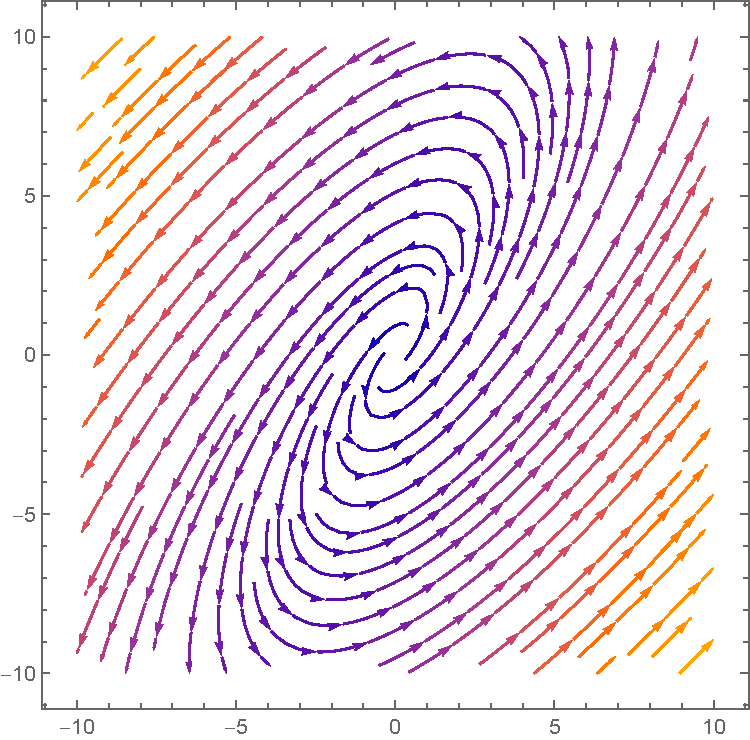
\includegraphics[width=0.4\textwidth]{Homework_3_Images/HW_3_Q1c.pdf}
    \end{figure}
    \vspace{12cm}


\item[d)] $\mathbf{x'} = \begin{pmatrix} 2 & -\frac{5}{2} \\ \frac{9}{5} & -1 \end{pmatrix} \mathbf{x}$\\
    $\left| \begin{array}{cc} 2 - \lambda & -\frac{5}{2}\\ \frac{9}{5} & -1 - \lambda\end{array}\right| 
    = (2 - \lambda)(-1 - \lambda) - (-\frac{5}{2})(\frac{9}{5}) = 0 \\\\
    \hspace*{95pt} = -2 - 2\lambda + \lambda + \lambda^2 + \frac{9}{2} = 0 \\\\
    \hspace*{95pt} = \lambda^2 - \lambda + \frac{5}{2} = 0 \\\\
    \hspace*{95pt} \Rightarrow \lambda_1 = \frac{1}{2}+\frac{3}{2}i, \lambda_2 = \frac{1}{2}-\frac{3}{2}i$

    \subsubsection*{Eigenvalue \#1}
    $\mathbf{\lambda_1 = \dfrac{1}{2}+\dfrac{3}{2}i}: 
    \left[\begin{array}{cc} 2 - \lambda_1 & -\frac{5}{2}\\ \frac{9}{5} & -1 - \lambda_1\end{array}\right]
    \rightarrow \left[\begin{array}{cc} \frac{3}{2}-\frac{3}{2}i& -\frac{5}{2}\\ \frac{9}{5} & -\frac{3}{2}-\frac{3}{2}i \end{array}\right] \left[\begin{array}{cc} v_1 \\ v_2 \end{array}\right] = \left[\begin{array}{cc} 0 \\ 0 \end{array}\right]$

    $\hspace*{2.2cm}\begin{array}{rr} (\frac{3}{2}-\frac{3}{2}i)v_1 - \frac{5}{2}v_2 &=0 \\ \frac{9}{5}v_1 - (-\frac{3}{2}+\frac{3}{2}i)v_2 &=0 \end{array} 
     \rightarrow \quad (3-3i)v_1=5v_2 \quad \rightarrow \mathbf{v}_1 =\left[\begin{array}{cc} 5 \\ 3-3i \end{array}\right]$

    So our general solution is $\mathbf{x} = c_1\begin{pmatrix} 5 \\ 3-3i \end{pmatrix}e^{(\frac{1}{2}+\frac{3}{2}i)t}$ \\
    This just looks bad and its hard to interpret, so let's use Euler's formula to rewrite it in a better way: \\
    $\begin{pmatrix} 5 \\ 3-3i \end{pmatrix}e^{(\frac{1}{2}+\frac{3}{2}i)t} = \begin{pmatrix} 5 \\ 3-3i \end{pmatrix}e^{\frac{1}{2}t}e^{\frac{3}{2}it}
    = \begin{pmatrix} 5 \\ 3-3i \end{pmatrix}e^{t}(\cos(\frac{3}{2}t) + i\sin(\frac{3}{2}t)) \\\\
    = e^{t}\left[\begin{pmatrix} 5(\cos(\frac{3}{2}t)+i\sin(\frac{3}{2}t)) \\ (3-3i)(\cos(\frac{3}{2}t)+i\sin(\frac{3}{2}t)) \end{pmatrix}\right] \\
    = e^{t}\left[\begin{pmatrix} 5\cos(\frac{3}{2}t) \\ 3\cos(\frac{3}{2}t) + 3\sin(\frac{3}{2}t) \end{pmatrix} + i\begin{pmatrix} 5\sin(\frac{3}{2}t) \\ 3\sin(\frac{3}{2}t) - 3\cos(\frac{3}{2}t) \end{pmatrix}\right] \\
    = c_1e^{t}\left[\begin{pmatrix} 5\cos(\frac{3}{2}t) \\ 3\cos(\frac{3}{2}t) + 3\sin(\frac{3}{2}t) \end{pmatrix}\right] + c_2e^{t}\left[\begin{pmatrix} 5\sin(\frac{3}{2}t) \\ 3\sin(\frac{3}{2}t) - 3\cos(\frac{3}{2}t) \end{pmatrix}\right] \\
    = c_1e^t \left[\begin{pmatrix} 5 \\ 3 \end{pmatrix} \cos(\frac{3}{2}t) - \begin{pmatrix} 0 \\ -3 \end{pmatrix} \sin(\frac{3}{2}t) \right] + c_2e^t \left[ \begin{pmatrix} 0 \\ -3 \end{pmatrix} \cos(\frac{3}{2}t) + \begin{pmatrix} 5 \\ 3 \end{pmatrix} \sin(\frac{3}{2}t)\right]$
    \\\\\\
    Notice that the vectors in front of the sins and cosines are components of the eigenvector that we started with:
    
    $$\mathbf{v}_1 =\left[\begin{array}{cc} 5 \\ 3-3i \end{array}\right] =\left[\begin{array}{cc} 5 \\ 3 \end{array}\right] + i\left[\begin{array}{cc} 0 \\ -3 \end{array}\right]$$
    
    This is a spiral source, so all trajectories will spiral outwards from the origin.
    \\\\
    Notice that with another example, our hypothesized shortcut still works! This is pretty cool, so maybe we can just use this formula for any complex eigenvalues we get in the future and save ourselves a lot of time!
    \begin{figure}[H]
        \centering
        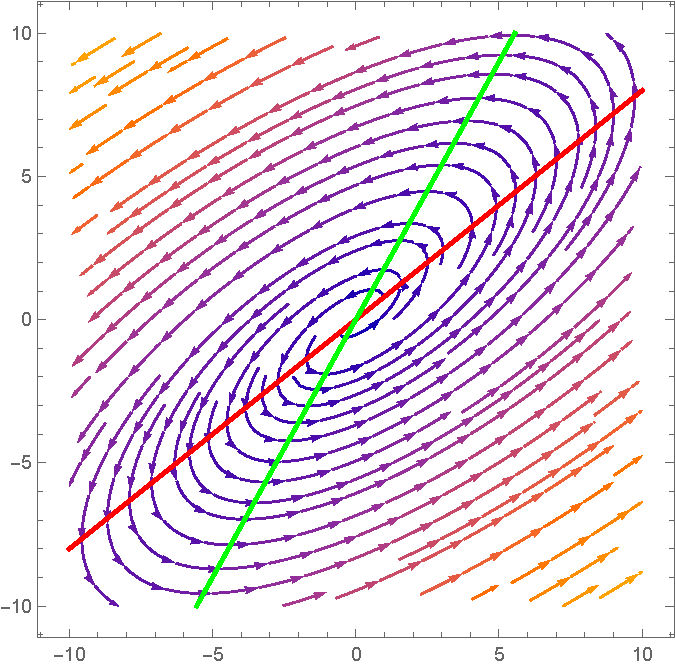
\includegraphics[width=0.4\textwidth]{Homework_3_Images/HW_3_Q1d.pdf}
    \end{figure}
\end{enumerate}

\vspace{10cm}
\section*{Question 2:}
Find the general solution of the 3D System:
\renewcommand{\arraystretch}{1}
$$\mathbf{x'}(t) = \begin{pmatrix} 1 & 1 & 2 \\ 1 & 2 & 1 \\ 2 & 1 & 1 \end{pmatrix} \mathbf{x}(t)$$

$\left| \begin{array}{ccc} 1-\lambda & 1 & 2\\ 1 & 2-\lambda & 1 \\ 2 & 1 & 1-\lambda\end{array}\right|
= (1-\lambda)\left| \begin{array}{cc} 2-\lambda & 1\\ 1 & 1-\lambda\end{array}\right| - 1\left| \begin{array}{cc} 1 & 1 \\ 2 & 1-\lambda\end{array}\right| +2\left| \begin{array}{cc} 1 & 2-\lambda\\ 2 & 1\end{array}\right|$ \\
$\hspace*{115pt} = (1-\lambda)\left[(2-\lambda)(1-\lambda) - 1\right] - 1[(1-\lambda) - 2] + 2[1-2(2-\lambda)]=0$ \\\\
$\hspace*{115pt} = (1-\lambda)(1-3\lambda + \lambda^2) + (1+\lambda) + (-6+4\lambda)=0$ \\\\
$\hspace*{115pt} = 1 - 3\lambda + \lambda^2 - \lambda + 3\lambda^2 -\lambda^3 -5 + 5\lambda = 0$ \\\\
$\hspace*{115pt} = -\lambda^3 + 4\lambda^2 + \lambda - 4 = 0$ \\\\
$\hspace*{115pt} = \lambda^3 - 4\lambda^2 - \lambda + 4 = 0$ \\\\
$\hspace*{115pt} = (\lambda^3 - 4\lambda^2) - (\lambda - 4) = 0$ \\\\
$\hspace*{115pt} = \lambda^2(\lambda - 4) - (\lambda - 4) = 0$ \\\\
$\hspace*{115pt} = (\lambda^2 - 1)(\lambda - 4) = 0$ \\\\
$\hspace*{115pt} \text{So our eigenvalues are: } \lambda_1 = 4, \lambda_2 = 1, \lambda_3 = -1$\\

\vspace{10cm}
\subsubsection*{Eigenvalue \#1}
$\mathbf{\lambda_1 = \phantom{-}3}: 
      \left[ \begin{array}{ccc} 1 & 2 & 3\\4 & 5 & 6 \\ 7 & 8 & 9\end{array}\right]
    = \left[ \begin{array}{ccc} 1 & 2 & 3\\4 & 5 & 6 \\ 7 & 8 & 9\end{array}\right]
    \xrightarrow{\text{RREF}} \left[ \begin{array}{ccc} 1 & 2 & 3\\4 & 5 & 6 \\ 7 & 8 & 9\end{array}\right]$\\ 

$\hspace*{1.5cm}$ This gives us that $\left\{\begin{array}{rl} a &= -c \\ b &= c \\ c &= c \end{array}\right.$
  so our eigenvalue is  $\mathbf{u}_1 = \left[ \begin{array}{c} 1\\ 2\\ 3\end{array}\right]$

\subsubsection*{Eigenvalue \#2}
$\mathbf{\lambda_2 = \phantom{-}1}: 
      \left[ \begin{array}{ccc} 1 & 2 & 3\\4 & 5 & 6 \\ 7 & 8 & 9\end{array}\right]  
    = \left[ \begin{array}{ccc} 1 & 2 & 3\\4 & 5 & 6 \\ 7 & 8 & 9\end{array}\right]   
    \xrightarrow{\text{RREF}} \left[ \begin{array}{ccc} 1 & 2 & 3\\4 & 5 & 6 \\ 7 & 8 & 9\end{array}\right]$\\ 

$\hspace*{1.5cm}$ This gives us that $\left\{\begin{array}{rl} a &= 0 \\ b &= -c \\ c &= c \end{array}\right.$
  so our eigenvalue is  $\mathbf{u}_2 = \left[ \begin{array}{c} 1\\ 2\\ 3\end{array}\right]$

\subsubsection*{Eigenvalue \#3}
$\mathbf{\lambda_3 = \phantom{-}0}: 
      \left[ \begin{array}{ccc} 1 & 2 & 3\\4 & 5 & 6 \\ 7 & 8 & 9\end{array}\right]    
    = \left[ \begin{array}{ccc} 1 & 2 & 3\\ & 5 & 6 \\ 7 & 8 & 9\end{array}\right]
    \xrightarrow{\text{RREF}} \left[ \begin{array}{ccc} 1 & 2 & 3\\4 & 5 & 6 \\ 7 & 8 & 9\end{array}\right]$\\ 

$\hspace*{1.5cm}$ This gives us that $\left\{\begin{array}{rl} a &= -c \\ b &= c \\ c &= c \end{array}\right.$
  so our eigenvalue is  $\mathbf{u}_3 = \left[ \begin{array}{c} 1\\ 2\\ 3\end{array}\right]$\\



\section*{Question 3:}
\begin{enumerate}
    \item[a)]
    \item[b)]
\end{enumerate}

\section*{Question 4:}
\begin{enumerate}
    \item[a)]
    \item[b)]
    \item[c)]
\end{enumerate}

\end{document}d\4